\documentclass[border=5mm]{standalone}
\usepackage{tikz}
\usepackage{tikz-qtree}

\begin{document}
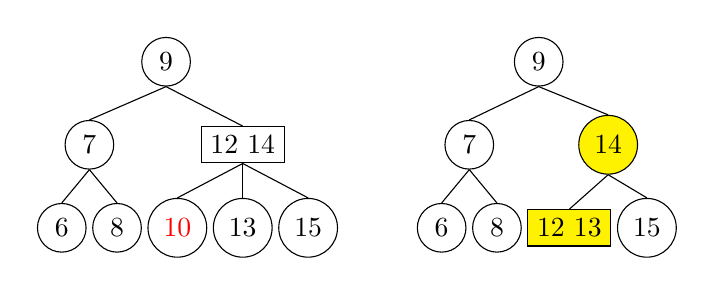
\begin{tikzpicture}[every tree node/.style={align=center}]
    \matrix[row sep=1cm, column sep=1cm] {
    \Tree
    [.\node[draw, circle]{9};
    [.\node[draw, circle]{7};
    [.\node[draw, circle]{6}; ]
    [.\node[draw, circle]{8}; ]
    ]
    [.\node[draw, rectangle]{12 14};
    [.\node[draw, circle]{\textcolor{red}{10}}; ]
    [.\node[draw, circle]{13}; ]
    [.\node[draw, circle]{15}; ]
    ]
    ];
    &
    \Tree
    [.\node[draw, circle]{9};
    [.\node[draw, circle]{7};
    [.\node[draw, circle]{6}; ]
    [.\node[draw, circle]{8}; ]
    ]
    [.\node[draw,fill=yellow, circle]{14};
    [.\node[draw,fill=yellow, rectangle]{12 13}; ]
    [.\node[draw, circle]{15}; ]
    ]
    ]; \\
    };
\end{tikzpicture}
\end{document}
